% --------------------------------------
% Document Class
% --------------------------------------
\documentclass[a4paper,11pt]{article}
% --------------------------------------



% --------------------------------------
% Use Package
% --------------------------------------


\usepackage[francais]{babel}
%\usepackage{ucs}
\usepackage[utf8]{inputenc}
\usepackage[T1]{fontenc}

\usepackage{makeidx}
\usepackage{color}
\usepackage{graphicx}
\usepackage{float}
\usepackage[hidelinks]{hyperref} 
\usepackage{geometry}
%\usepackage{lastpage}
%\usepackage{marginnote}
\usepackage{fancyhdr}
%\usepackage{titlesec}
%\usepackage{framed}
\usepackage{amsmath}
\usepackage{empheq}
\usepackage{array}
\usepackage{multicol}
%\usepackage{adjustbox}

% insert code
\usepackage{listings}

% define our color
\usepackage{xcolor}

% code color
\definecolor{ligthyellow}{RGB}{250,247,220}
\definecolor{darkblue}{RGB}{5,10,85}
\definecolor{ligthblue}{RGB}{1,147,128}
\definecolor{darkgreen}{RGB}{8,120,51}
\definecolor{darkred}{RGB}{160,0,0}

% other color
\definecolor{ivi}{RGB}{141,107,185}


\lstset{
    language=Scilab,
    captionpos=b,
    extendedchars=true,
    frame=lines,
    numbers=left,
    numberstyle=\tiny,
    numbersep=5pt,
    keepspaces=true,
    breaklines=true,
    showspaces=false,
    showstringspaces=false,
    breakatwhitespace=false,
    stepnumber=1,
    showtabs=false,
    tabsize=3,
    basicstyle=\small\ttfamily,
    backgroundcolor=\color{ligthyellow},
    keywordstyle=\color{ligthblue},
    morekeywords={include, printf, uchar},
    identifierstyle=\color{darkblue},
    commentstyle=\color{darkgreen},
    stringstyle=\color{darkred},
}


% --------------------------------------



% --------------------------------------
% Page setting
% --------------------------------------
%\pagestyle{empty}
\setlength{\headheight}{15pt}

\setcounter{secnumdepth}{3}
\setcounter{tocdepth}{2}

\makeatletter
\@addtoreset{chapter}{part}
\makeatother 

\hypersetup{         % parametrage des hyperliens
  colorlinks=true,      % colorise les liens
  breaklinks=true,      % permet les retours à la ligne pour les liens trop longs
  urlcolor= blue,       % couleur des hyperliens
  linkcolor= black,     % couleur des liens internes aux documents (index, figures, tableaux, equations,...)
  citecolor= green      % couleur des liens vers les references bibliographiques
}

% --------------------------------------

% --------------------------------------
% Information
% --------------------------------------
\title{Compte-rendu TP1 TI : Sources lumineuses}
\author{Elliot VANEGUE et Gaëtan DEFLANDRE}
% --------------------------------------

\definecolor{myColor}{rgb}{0.5, 0.1, 0.75}

% --------------------------------------
% Begin content
% --------------------------------------
\begin{document}

% Set language to english
  \selectlanguage{francais}

  % Start the page counting
  \pagenumbering{arabic}

  \maketitle
  
  \mbox{}
  \newpage
  \clearpage
  
  \section*{Introduction}
  Pour ce premier TP, nous nous sommes initiés à l'outil Scilab qui permet d'effectuer facilement des opérations matricielles 
  et de les afficher dans un graphique. Nous avons utilisé cet outil pour simuler l'éclairement d'une surface à l'aide de 
  différentes sources lumineuses. Le but de ce TP est d'étudier les sources ponctuelles isotrope et lambertienne.
  Nous allons chercher à optimiser l'éclairement sur une surface via plusieurs sources lumineuses.
  
  \section{Eclairement d'une source ponctuelle isotrope}
  Une source ponctuelle isotrope émet la même intensité énergétique dans toutes les 
  directions. Nous allons voir comment calculer l'éclairement sur une surface
  avec cette source lumineuse.\\
  
  Nous avons modifié le code en exemple afin de calculer les valeurs d'éclairement de 
  chaque élément de la surface par une source lumineuse isotrope. Nous obtenons le code 
  suivant :
  
  \begin{lstlisting}[caption=Code Scilab eclairement source isotrope]
  // Definition des echantillons sur un axe
  axe = [0:99] / 100 + 5e-3;
  // Definition des elements de surface
  x = ones (1:100)' * axe;
  y = axe' * ones (1:100);
  // Position de la source -> sur le plan
  xs = 0.5;
  ys = 0.5;
  // Puissance
  Phi=100;

  // Calcul de la distance
  d = sqrt ((x - xs).^2 + (y - ys).^2);

  // Intensite energetique
  I0=Phi/2/%pi;

  // Hauteur
  h= 0.5;

  // Eclairement
  e = I0 * (h .* ((h^2 + d.^2).^(-3/2)));
  plot3d (axe, axe, e);
  imshow (e/max(e));
  \end{lstlisting}
  \newpage
  
  Soit le calcul de l'éclairement:
  
  \begin{empheq}[box=\fbox]{align}
  \Phi &= 100 W \nonumber\\
  cos(\theta) &= \frac{h}{\sqrt{h^{2}+d^{2}}} \nonumber\\
  E(P) &= \frac{\Phi}{(h^{2}+d^{2})*2\pi}*cos(\theta)\nonumber
  \end{empheq}
  
  
  Avec ce calcul nous obtenons une courbe comme celle-ci :
  
  \begin{figure}[H]
    \center
    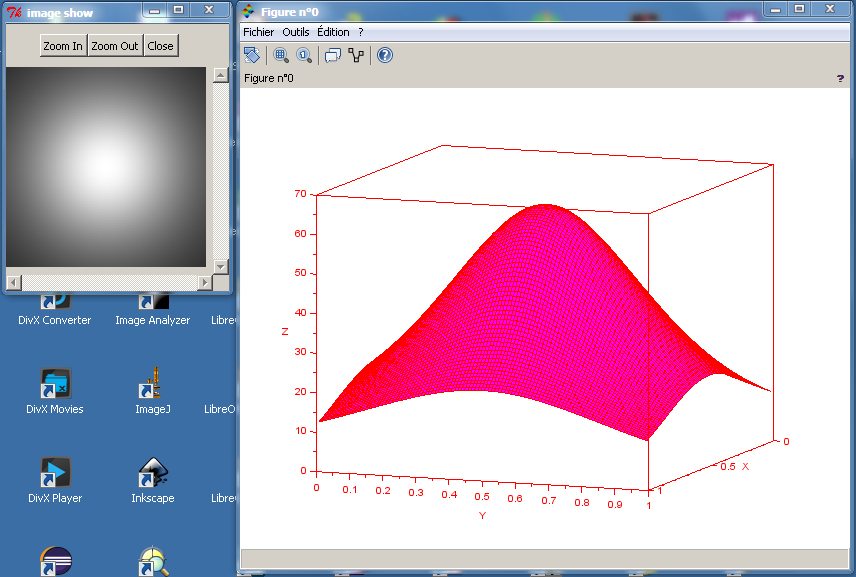
\includegraphics[width=10cm]{../isotrope.PNG}
    \caption{Graphique de la répartition de la lumière d'une source isotrope}
  \end{figure}
  
  Sur ce graphique, nous pouvons voir que l'intensité de la lumière est plus 
  importante sur la surface lorsque l'on se trouve proche de la normale de la source.
  De plus, l'éclairement reçu par la surface diminue sur les bords de celle-ci.

  \section{Eclairement d'une source ponctuelle lambertienne}
  Une source lambertienne adopte un schéma un peu différent d'une source ponctuelle isotrope.
  Le diagramme d'émission de cette source varie en fonction du cosinus de l'angle d'émission.
  
  \begin{figure}[H]
    \center
    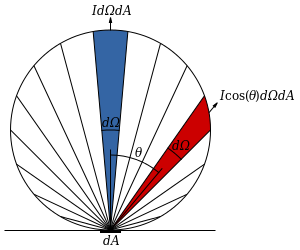
\includegraphics[width=7cm]{../Lambert_Cosine_Law_1.png}
    \caption{Représentation d'une source lumineuse isotrope lambertienne}
  \end{figure}
  
  Nous avons à nouveau modifié le code afin de prendre en compte cette dispersion de la 
  lumière. Nous obtenons le calcul suivant :
  
  $$ E(P)=\frac{\Phi}{(h^{2}+d^{2})*2\pi}*cos(\theta)^{2} $$\\
  
  Voici le code correspondant à l'expression ci-dessus :
  
  \begin{lstlisting}[caption=Nouvelle eclairement pour une source lambertienne]
  // Eclairement avec source de lambert
  e = I0 * ((h^2) .* ((h^2 + d.^2).^(2)).^(-1))
  \end{lstlisting}
  
  Ici nous voyons que l'exposant du dénominateur a changé, car pour une source lambertienne, 
  le cosinus de l'angle theta intervient deux fois.
  \begin{itemize}
    \item Une première fois, comme pour la source isotrope, la source ponctuelle émet dans toutes 
    les directions. Donc les rayons, qui ont pour direction la normale de la source arrivent plus 
    directement sur la surface de l'objet. Plus l'angle par rapport à la normale de la source grandit, 
    plus la distance que les rayons devront parcourir sera grande.
    \item Une seconde fois, car dans le cas de la source lambertienne, plus l'angle par rapport 
    à la normale augmente, plus l'éclairement diminue, en fonction du cosinus de cet angle 
    (\textit{cf FIGURE 2}).\\
  \end{itemize}
  
  \begin{figure}[H]
    \center
    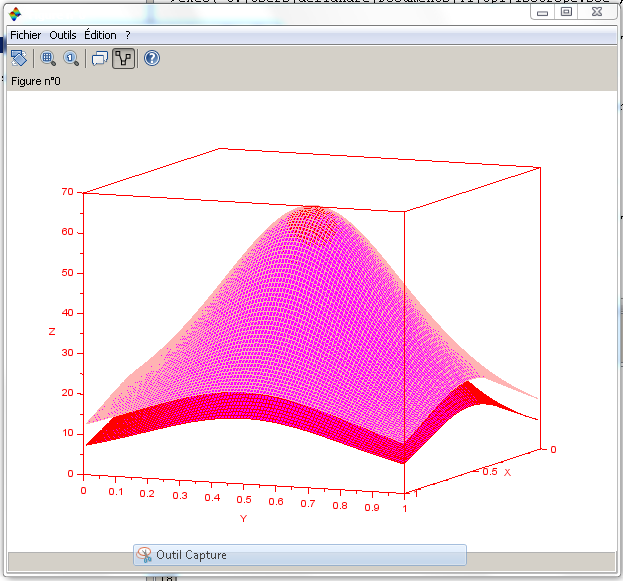
\includegraphics[width=10cm]{../iso_lamb.PNG}
    \caption{Graphique des sources ponctuelles (rose claire) et lambertienne (rose foncé)}
  \end{figure}
  
  Ce calcul nous donne une courbe avec une pente plus importante, car la lumière éclaire moins les 
  bords de la surface par rapport à une source ponctuelle isotrope. En effet, l'éclairement d'une 
  source de Lambert décroît plus vite lorsque l'angle $\theta$ est grand.
  
  \section{Eclairement d'une grille de source ponctuelle}
  
  Nous allons maintenant disposer plusieurs sources lambertiennes de manière à minimiser la
  variance quel que soit le nombre de sources. Il faut positionner sur une grille de \textbf{N*N}
  sources \textbf{régulièrement espacées}. Pour cette simulation, nous avons une surface de $1m^{2}$
  qui doit être éclairée avec une grille de source lumineuse de $4m^{2}$.\\
  
  \begin{figure}[H]
    \center
    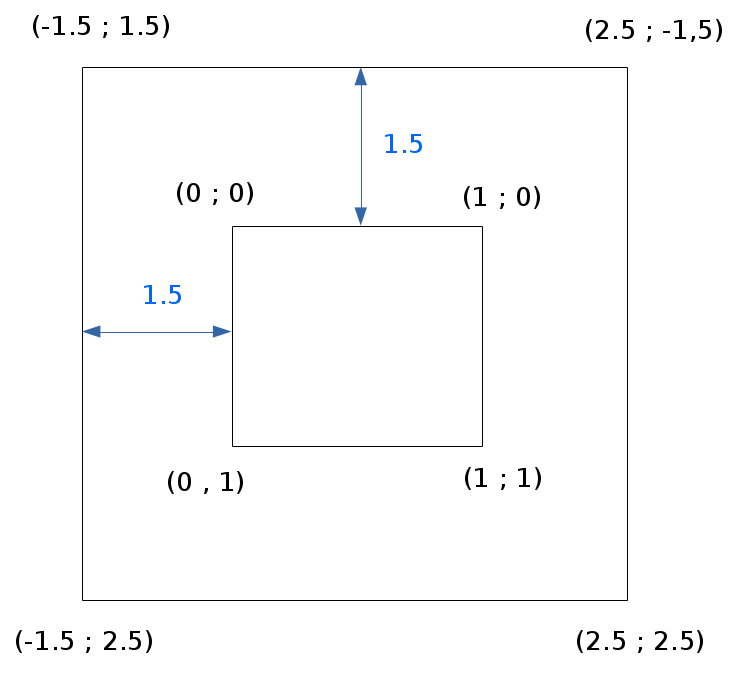
\includegraphics[width=10cm]{../schema.png}
    \caption{Schéma de la disposition de la surface (petit carré) et de la grille de source (grand carré)}
  \end{figure}
  
  Pour effectuer cette simulation, nous avons écrit le code suivant :\\
  
  \begin{lstlisting}[caption=Code pour l'eclairement d'une grille de sources ponctuelles]
    // Définition des échantillons sur un axe
    axe = [0:99] / 100 + 5e-3; 
    // Définition des éléments de surface
    x = ones (1:100)' * axe;
    y = axe' * ones (1:100);

    // Grille de N*N source
    N = 10;

    // Hauteur
    h = 0.5;

    // Puissance
    Phi = 100;

    // Création de la liste des positions des sources
    lxs = list();
    lys = list();
    nbSource = 0;

    xmin = -1.5
    xmax = 2.5
    ymin = -1.5
    ymax = 2.5
    ecartx = abs(xmin) + abs(xmax)
    ecarty = abs(ymin) + abs(ymax)

    pasx = ecartx / (N-1)
    pasy = ecarty / (N-1)

    for i = 1:N
        for j = 1:N
            nbSource = nbSource + 1;
            lxs(nbSource) = xmin + pasx * (i-1);
            lys(nbSource) = ymin + pasy * (j-1);
        end;
    end;

    // Calcul des distances de chaque element pour chaque source
    ld = list();
    for i = 1:nbSource
	xs = lxs(i);
	ys = lys(i);
	ld(i) = sqrt ((x - xs).^2 + (y - ys).^2);
    end;

    // Intensite energetique
    I0=Phi/2/%pi;

    e = list();

    for i = 1:nbSource
	e(i) = I0 * ((h^2) .* ((h^2 + ld(i).^2).^(2)).^(-1));
    end;

    sume = e(1); 
    for i = 2:nbSource
	sume = e(i) + sume;
    end;

    variation = ((max(sume) - min(sume)) * 100) / max(sume);
    
    disp(variation);
    plot3d (axe, axe, sume);
  \end{lstlisting}
  
  \newpage
  
  Nous avons ensuite recherché combien de sources lumineuses seraient suffisantes pour avoir
  une variation relative de l'éclairement inférieur à 5\%. Nous avons obtenu les résultats 
  suivants :
  
 \begin{center}
    \begin{tabular}{|c|c|c|}
      \hline
      \textbf{Valeur de N} & \textbf{Variance (\%)} & \textbf{Image}\\
      \hline
      2 & 22.819947 & 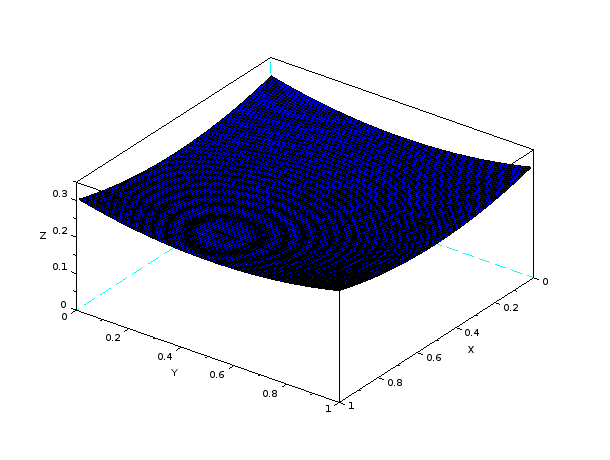
\includegraphics[width=4cm]{../grille2.png}\\
      \hline
      5 & 57.345498 & 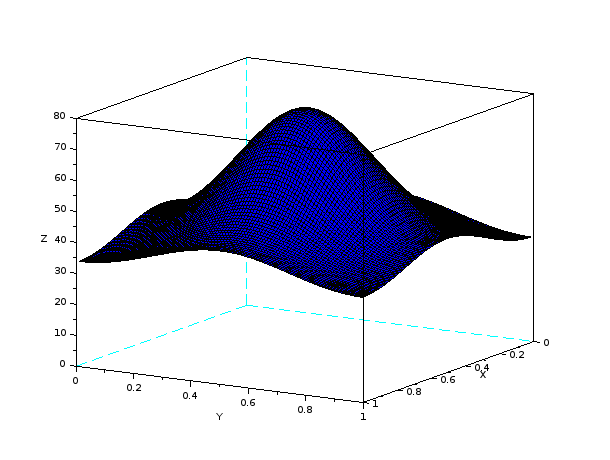
\includegraphics[width=4cm]{../grille5.png}\\
      \hline
      8 & 9.9139412 & 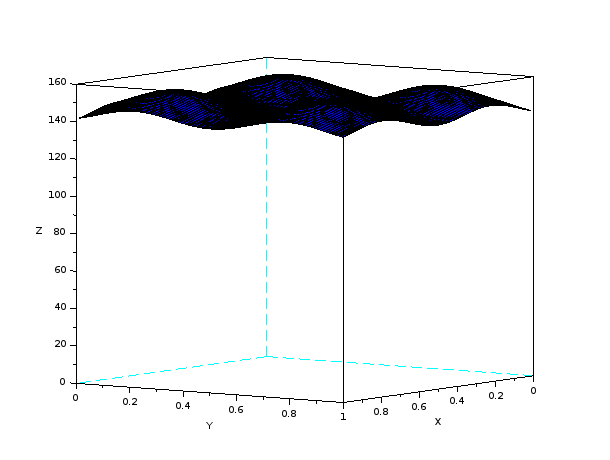
\includegraphics[width=4cm]{../grille8.png}\\
      \hline
      9 & 5.1679987 & 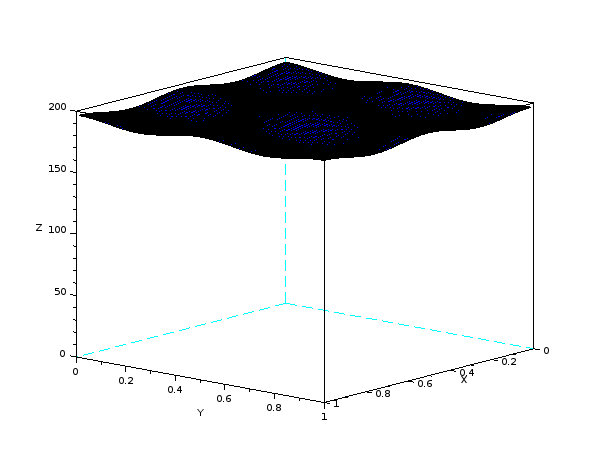
\includegraphics[width=4cm]{../grille9.png}\\
      \hline
      10 & 2.8661993 & 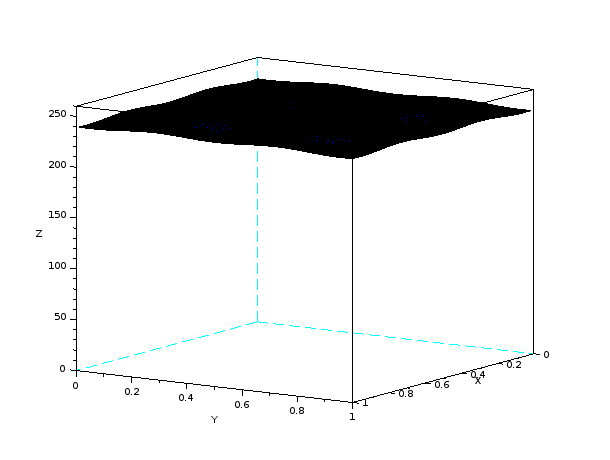
\includegraphics[width=4cm]{../grille10.png}\\
      \hline
    \end{tabular}
  \end{center}
  
  Ces résultats montrent que la variation relative de l'éclairement ne dépend pas que du nombre 
  de sources lumineuses, mais aussi du positionnement de celles-ci. On voit que la variance avec 
  deux sources est plus petite que la variance avec cinq, alors que les valeurs qui suivent décroissent.
  
  \section*{Conclusion}
  En conclusion, nous avons vu que l'éclairement d'une scène dépend de nombreux paramètres. L'exemple 
  des sources isotropes montre que cela dépend de l'intensité de la source lumineuse et de la distance 
  entre la source et l'objet. Alors que dans le cas d'une source lambertienne, nous avons remarqué qu'en 
  plus de dépendre de ces paramètres, cela varie avec l'angle d'émission.
  Enfin, nous avons vu avec l'exemple d'une grille de sources que la variance relative de l'éclairement 
  d'une scène dépend du nombre de sources, mais aussi de leurs positionnements.
    
\end{document}